
\subsection{Pregel: Bulk Synchonous Parallel}
Much  of  the  mismatch  stems  from  the  lack  of  shared  global  state.
Complex  applications  and  interactive  queries  both  need  one  thing  that
MapReduce lacks: efficient  primitives  for  data  sharing.


With \textbf{Pregel}, we consider the  nodes  with a  state  (memory)  
that  carries  from  superstep to  superstep.

\subsubsection{Model}

It's a sequence of \textbf{superstep} where at superstep $S$:
\begin{enumerate}
    \item Compute in parallel at each $V$
        \begin{itemize}
            \item Read message sent to $V$ in $S-1$
            \item Update value/state
            \item Optionnaly change topology
        \end{itemize}
    \item Send messages to neighbors
    \item Synchronization
\end{enumerate}

\begin{tabular}{m{9cm}m{7cm}}
    $\rightarrow $ Algorithm terminates when all vertices are simultaneously inactive.
    & 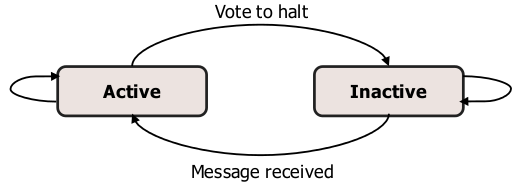
\includegraphics[width=7cm]{img/halt}
\end{tabular}

\subsubsection{Algorithm}
\begin{itemize}
    \item \textbf{Find Maximum Value}

        \begin{tabular}{m{11cm}m{5cm}}
            \begin{enumerate}
                \item At superstep 0, propagating value to neighbors
                \item In each step, if he learn a larger number, then propagate
                    it to neighbors else vote to halt
                \item Finish when all vote halt
            \end{enumerate}
            & 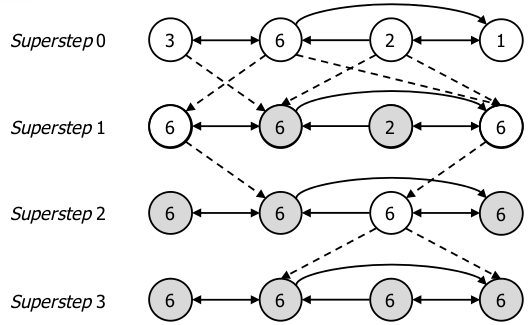
\includegraphics[width=5cm]{img/FMV}
        \end{tabular}

    \item \textbf{PageRank}
        $$rank_i = 1-d + d \sum_{j \in B_i} \frac{1}{N_j} rank_j \quad \textrm{where }N_i \textrm{ is
        the outgoing link of i and} B_i \textrm{ the ingoing link of i}$$ 

        \begin{itemize}
            \item Each  page  $j$  distributes  its  importance  to  all  of  the  pages  it  
                points  to  (so  we  scale  by  $\frac{1}{N_j}$)
            \item Page  p’s  importance  is  increased  by  the  importance  of  its  
                back  set
        \end{itemize}
        %TODO: example pregel code ?

\end{itemize}


\subsection{Spark: Resilient Distributed Dataset}

Basically, Spark is a distributed  memory  abstraction  that  is  both  fault-­tolerant  
and  efficient. Note that there is some restriction form of distributed shared memory
in order to be called \textit{Resilient Distributed Datasets (RDDs)}
\begin{itemize}
    \item Immutable, partitioned collections of records
    \item Can  only  be  built  through  coarse-­grained deterministic  
        transformations  (map,  filter,  join,  ...)
\end{itemize}

Despite their restrictions,  RDDs can express many parallel algorithms (These
naturally  apply the same operation to many items). RDDs also unify many
programming models.

\begin{tabular}{m{7cm}cm{7cm}}
    \begin{itemize}
        \item MapReduce,  DryadLINQ
        \item Pregel graph  processing
        \item Iterative  MapReduce
        \item SQL:  Hive  on  Spark  (Shark)
    \end{itemize}
    & $\Rightarrow$  &
    All are based on coarse-­grained  
    operations
\end{tabular}

\begin{center}
    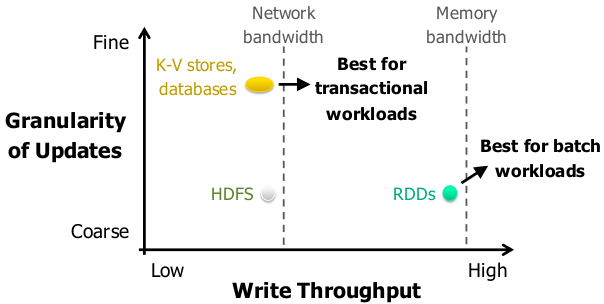
\includegraphics[width=11cm]{img/databaseComp}
\end{center}

\subsubsection{Efficient fault recovery}
Spark use \textbf{lineage}:

\begin{tabular}{m{9cm}m{7cm}}
    \begin{itemize}
        \item Log  one  operation  to  apply  to  many  elements
        \item Recompute lost  partitions  on  failure
        \item No  cost  if  nothing  fails
    \end{itemize}
    &
    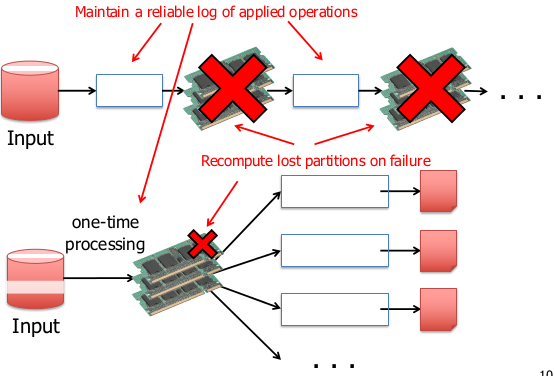
\includegraphics[width=7cm]{img/sparkFault}
\end{tabular}

\subsubsection{Spark operation}
\begin{itemize}
    \item Transformations (define a new RDD) : \begin{tabular}{ccc}
            map & flatMap & union \\ join & cogroup & cross \\ mapValues & filter & sample\\
            groupByKey & reduceByKey& sortByKey\\
        \end{tabular}

    \item Action (return a result to driver program) : \begin{tabular}{ccc}
            collect& reduce& count\\ save& lookupKey& take\\
        \end{tabular}
\end{itemize}

\subsubsection{Spark scheduler}

\begin{tabular}{m{7cm}m{8cm}}
    \begin{itemize}
        \item Pipelines  functions within  a  stage
        \item Locality  \&  data  reuse aware
        \item Partitioning-­aware to  avoid  shuffles
    \end{itemize}
    &
    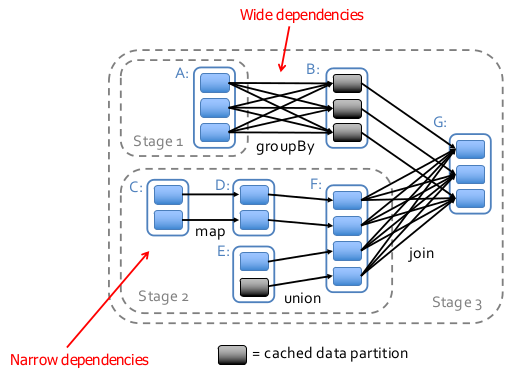
\includegraphics[width=8cm]{img/sparkScheduler}
\end{tabular}

\subsubsection{Algorithm}
\begin{itemize}
    \item \textbf{PageRank}:
        $$rank_i = 1-d + d \sum_{j \in B_i} \frac{1}{N_j} rank_j \quad \textrm{where }N_i \textrm{ is
        the outgoing link of i and} B_i \textrm{ the ingoing link of i}$$ 

        \begin{lstlisting}[mathescape]
        var links   =  //  RDD  of  (url,   neighbors)   pairs
        var ranks   =  //  RDD  of  (url,   rank)   pairs
        for  (i $\leftarrow$ 1 to ITERATIONS)   {
            contribs =  links.join(ranks).flatMap {
                (url,   (links,   rank))   =>
                links.map(dest =>  (dest,   rank/links.size))
            }
            ranks   =  contribs.reduceByKey((x,   y)  =>  x  +  y)
            .mapValues(sum   =>  0.85*sum   +  0.15/N)
        }
        \end{lstlisting}
        Note that as RDDs are  immutable, contribs and  ranks  are  new  RDDs!

        %TODO optimizing placement slide 20 for 07
\end{itemize}


